%% LyX 2.1.2 created this file.  For more info, see http://www.lyx.org/.
%% Do not edit unless you really know what you are doing.
\documentclass[usenatbib]{emulateapj}
\usepackage[latin9]{inputenc}
\setcounter{secnumdepth}{3}
\setcounter{tocdepth}{3}
\usepackage{color}
\usepackage{amsmath}
\usepackage{graphicx}
\usepackage[unicode=true,pdfusetitle,
 bookmarks=true,bookmarksnumbered=false,bookmarksopen=false,
 breaklinks=true,pdfborder={0 0 0},backref=section,colorlinks=true]
 {hyperref}
\hypersetup{
 linkcolor=blue,citecolor=blue}

\makeatletter
%%%%%%%%%%%%%%%%%%%%%%%%%%%%%% Textclass specific LaTeX commands.
\newenvironment{lyxcode}
{\par\begin{list}{}{
\setlength{\rightmargin}{\leftmargin}
\setlength{\listparindent}{0pt}% needed for AMS classes
\raggedright
\setlength{\itemsep}{0pt}
\setlength{\parsep}{0pt}
\normalfont\ttfamily}%
 \item[]}
{\end{list}}

%%%%%%%%%%%%%%%%%%%%%%%%%%%%%% User specified LaTeX commands.
\usepackage[caption=false]{subfig}

\makeatother

\begin{document}
\title{The Fundamental Plane of Black Hole Activity in the Illustris Simulation}
\author{Diego F. Gonz\'alez-Casanova, Tim Haines, Zachary Pace, Brianna Smart, Andrea Vang}
\address{Astronomy Department, University of Wisconsin-Madison, 475 North Charter Street, Madison, WI 53706-1582, USA}
\begin{abstract}
Here is our abstract.
\end{abstract}
\keywords{black hole physics -- accretion -- cosmology: miscellaneous}
\maketitle


\section{Introduction}

Since the earliest simulations of the formation and evolution of disk
galaxies, the problem of stability of the gas in the disk has been
a key issue \citep[e.g., ][]{lucy1977anumerical}. One prominent example
of this is the so-called 'angular-momentum catastrophe' \citep{navarro1994accretion}
in which the specific angular momentum of simulated disks is smaller
than values observed in real galaxies by an order of magnitude- resulting
in disks with sizes smaller than observations by a similar factor.
Further, the gas in the simulated disks cools too quickly, causing
it to spiral into the disk's center and form a bulge. However, not
all disk galaxies contain a bulge. Clearly, then, the simulations
are not faithfully representing the physical processes governing disk
formation in nature. The currently accepted solution to this problem
is the introduction of one or more feedback mechanisms which deposit
energy into the gas, heating it, and preventing its aggregation in
the disk's center.

One popular mechanism to drive this feedback is the accretion of gas
onto a central black hole. These so-called active galactic nuclei
(AGN) are believed to be important in the evolution of galaxies as
a mechanism for quenching star formation \citep[see ][and references therein]{hopkins2008acosmological}
and stabilizing the gas disk \textbf{{[}CITATION{]}}. The presence
of AGN in $\sim3\%$ of local galaxies at $z\lesssim0.7$ \citep{haggard2010thefield}
with an increasing fraction at higher redshifts \citep{martini2013thecluster}
indicates that this mechanism may contribute a non-negligible source
of energy for evolving galaxies. Additionally, the invocation of an
AGN feedback mechanism has been shown to be necessary in order to
recreate the present-day color-magnitude relation of massive red galaxies
\citep{springel2005blackholes}. Thus, in order to understand galaxy
evolution, it is important to understand the physics governing black
hole accretion.

The question then remains as to how we can tie properties of AGN in
simulations back to observations to further constrain the physics
of this feedback mechanism. Fortunately, there are distinctive signatures
of AGN activity that can be used to probe for the presence of an accreting
black hole. For example, relativistic jets emitting synchrotron radiation
in the radio are a strong indicator of recent AGN activity \textbf{{[}CITATION{]}}.
Additionally, X-ray emission typically in excess $\sim10^{42}\,{\rm ergs}\,{\rm s^{-1}}$
stemming from inverse-Compton scattering of electrons in the corona
around the accretion disk of the black hole provides a clear signpost
of a strong source of ionizing energy. \citet[hereafter, M03]{merloni2003afundamental}
investigate the properties of $\sim100$ local galaxies containing
an AGN with compact emission in both the X-ray and radio and show
that the radio luminosity is well correlated both with the mass of
the central black hole and the galaxy's X-ray luminosity. In that
work, M03 define a fundamental plane combining the two observational
signatures (X-ray and radio luminosities) with the accretion flow
onto the black hole. The existence of the fundamental plane suggests
that the physical processes regulating the conversion of gas accreted
onto the black hole into radiative energy could be universal across
the entire scale of black hole masses.

Clearly, then, an important component of modern galaxy formation simulations
is the correct implementation of AGN feedback. In this work, we test
the accuracy of the AGN feedback mechanism in the state-of-the-art
hydrodynamical cosmological simulation Illustris-2. Specifically,
we aim to determine the fundamental plane of black hole activity using
the mass and accretion rates in the simulation and compare against
those measured in M03. From this analysis, we can begin to understand
how well state-of-the-art simulations replicate the real physics of
black hole accretion and AGN feedback in the universe to better understand
the relationship between AGN and the evolution of their host galaxies.

This paper is structured as follows. In Section \ref{sec:illustris},
we outline the implementation of the Illustris-2 simulations. Section
\ref{sec:sample} discusses our sample of black holes extracted from
Illustris-2. Section \ref{sec:analysis} we determine how the black
holes in the Illustris-2 simulation coincide with the fundamental
plane of M03. In Section~\ref{sec:discussion} we discuss our results,
and Section \ref{sec:conclusions} presents our final conclusions.


\section{The Illustris Simulation}

\label{sec:illustris}The Illustris Project is a series of large-scale
cosmological hydrodynamical simulations of galaxy formation \citep{vogelsberger2014properties}.
The simulation consists of large cosmological situations in a periodic
box with $106.5\;{\rm Mpc}$, simulated with different physics at
different resolutions. It assumes a standard flat $\Lambda$CDM cosmology
with $\Omega_{m,0}=0.2726$, $\Omega_{\Lambda,0}=0.72746$, $\Omega_{b,0}=0.0456$,
and $H_{0}=70.4$ km s$^{-1}$ Mpc$^{-1}$ from the Wilkinson Microwave
Anisotropy Probe 9-year data release \citep{hinshaw2013nineyear}.

In the Illustris simulations, collisionless black hole particles with
a seed mass of $1.42\times10^{5}M_{\odot}$ are placed in dark matter
halos of mass greater than $7.1\times10^{10}M_{\odot}$\citep{sijacki2014theillustris}.
The black hole seeds are allowed to grow through gas accretion or
through mergers with other black holes. The black hole seeds are allowed
to grow through gas accretion, parametrized in terms of Eddington
limited Bondi-Hoyle-Lyttleton (BHL)-like accretion (\citet{bondi1952accretion,bondihoyle1044}),
or through mergers with other black holes. BHL is a non-spherical
accretion flow which develops when a compact object moves relative
to a uniform gas cloud. The BHL accretion rate on the black hole is
given by

\begin{equation}
\dot{M}_{B}=\frac{4\pi G^{2}M_{BH}^{2}\rho}{(c_{s}^{2}+v^{2})^{3/2}},
\end{equation}


where $\rho$ and $c_{s}$ are the density and sound speed of the
gas, respectively, $\alpha$ is a dimensionless parameter, and $v$
is the velocity of the black hole relative to the gas. Then, the accretion
is limited to the Eddinton rate,

\begin{equation}
\dot{M}_{Edd}=\frac{4\pi G^{2}M_{BH}m_{p}}{\epsilon_{r}\sigma_{T}c},
\end{equation}


where $m_{p}$ is the proton mass, $\sigma_{T}$is the Thompson cross-section
and $\epsilon_{r}$is the radiative efficiency. The radiaitve efficiency
is related to the radiated bolometric luminosity, $L_{B}$, and accretion
rate, $\dot{M}_{BH}$, by
\begin{lyxcode}
\begin{equation}
\epsilon_{r}=\frac{L_{r}}{\dot{M}_{BH}}
\end{equation}

\end{lyxcode}
This simply gives the mass to energy conversion efficiency set by
the amount of energy that can be extracted from the innermost stable
orbit of an accretion disk around a black hole. At $z=0$, there are
32,542 black holes in total with 3965 black holes more massive than
$10^{7}M_{\odot}$.\textbf{Let's add some details about the BH prescription
so we can talk about it in the discussion.}


\section{Sample of Black Holes}

\label{sec:sample}The BH population in Illustris was analysed using
the low resolution simulation at a redshift of $z=0$. The Illustris
simulation gives the mass and accretion rate for each BH. We first
eliminate all BH particles with $M=0$ or $\dot{{\rm M}}=0$, which
we assume to be unphysical. We will hereafter refer to the remaining
population (admittedly somewhat anomalously) as the Full Illustris-2
Black Hole Sample. We argue that if accretion rate and X-ray luminosity
are indeed linearly related, accretion rates on the order of $\sim10^{-15.7}M_{\odot}s^{-1}$
and lower should not be detectable in the X-ray bands at cosmological
distances. \textbf{I know this is hand-wavey, I'll fix it later.}
Additionally, the presence of the low-accreting population skews the
$M-\dot{M}$ fit severely: since we are attempting to fit a linear
relationship, effectively between mass and accretion rate, such anomalously
low-accreting black holes should be omitted.

We accomplished this by first noting that the main sequence of black
holes follows roughly a log-normal distribution in accretion rate
space, centered around approximately $\dot{M}_{BH}=10^{-12.5}M_{\odot}/s$.
However, there also exists a small, secondary population centered
around approximately $\dot{M}_{BH}=10^{-15.7}M\odot/s$ (see Figure
\ref{fig:bhpop_mdot}). To produce a clean sample of accreting black
holes, we fit the Full Sample with two Gaussian profiles (in $\log\dot{M}$-space)
using astroML's one-dimensional Gaussian mixture \citep{vanderplas2012introduction},
and require an accretion rate of $\ge10^{-15.7}\; M_{\odot}yr^{-1}$
(the arithmetic mean of the low-accreting samle). This yields a total
of $23,277$ for our final sample black holes with masses $4.3\times10^{4.3}M_{\odot}\le M_{BH}\le5.85\times10^{10}M_{\odot}$.
\begin{figure}
\centering{}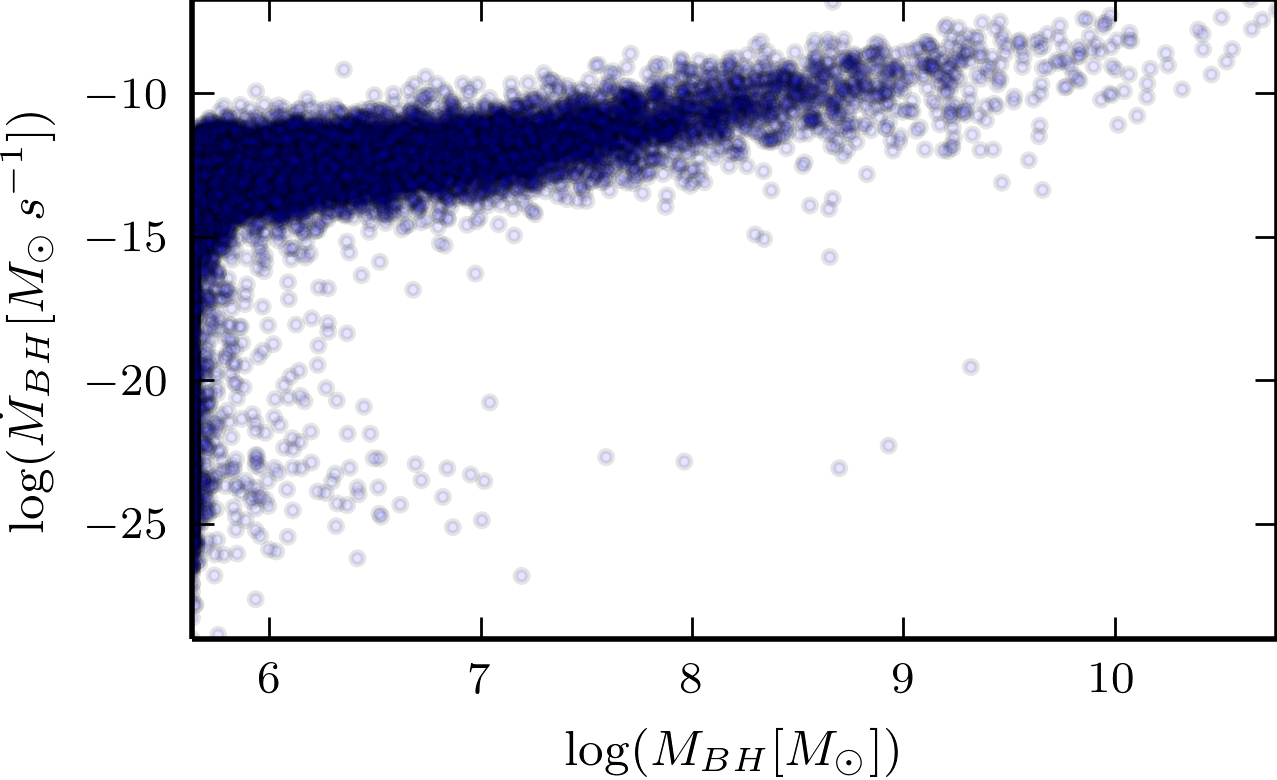
\includegraphics[clip]{Figures/Illustris2_bhpop_full}
\protect\caption{\label{fig:bhpop_full}The full Illustris-2 black hole sample in mass-accretion
rate space. Each light blue dot represents a single black hole with
mass in units of $M_{\odot}$ and accretion rate in units of $M_{\odot}s^{-1}$.}
\end{figure}
\begin{figure}
\centering{}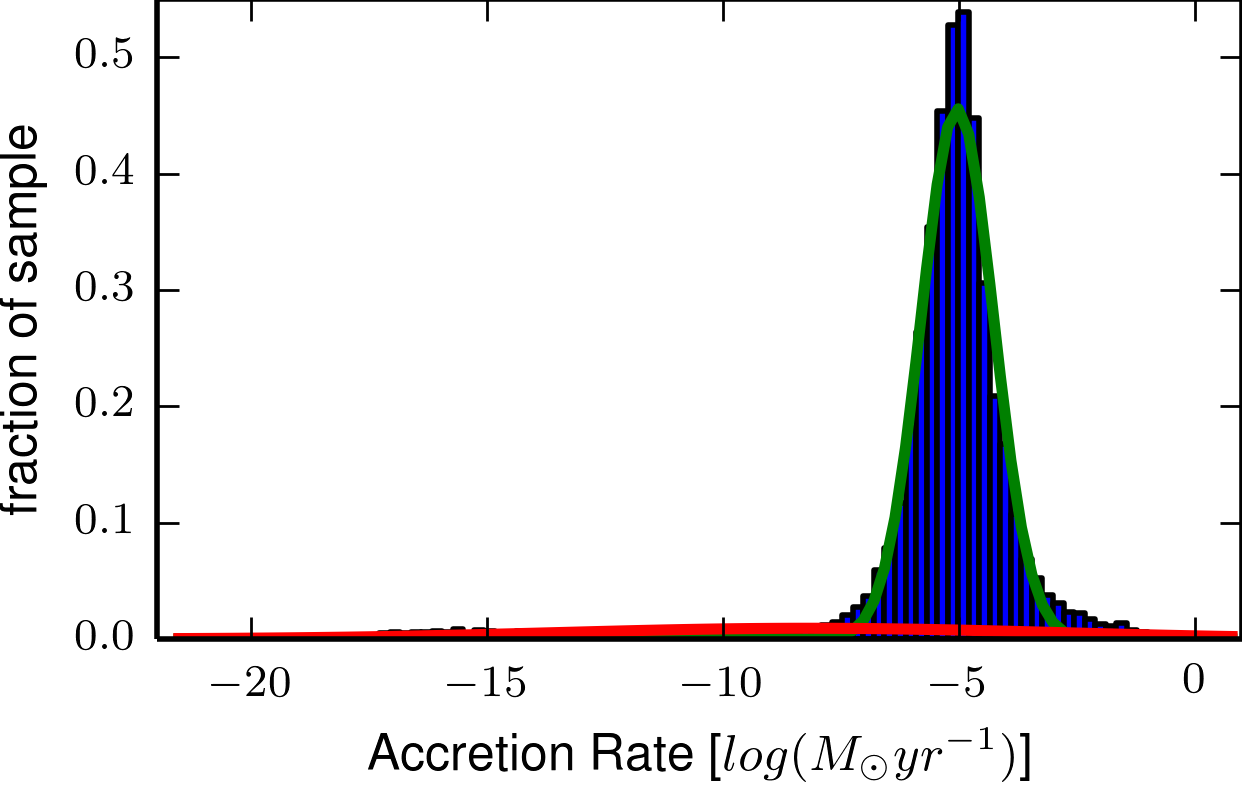
\includegraphics[clip]{Figures/Illustris2_bhpop_mdot}
\protect\caption{\label{fig:bhpop_mdot}The Full Sample exhibits a weak, but noticeable
bimodality in accretion rate space. We fit two log-normal distributions
to the raw distribution. The green Gaussian profile denotes the high-accreting
population, and the small, red Gaussian profile denotes the low-accreting
population. We impose a strict cutoff on the accretion rate at the
peak of the red profile, eliminating most of the anomalously low-accreting
population.}
\end{figure}



\section{Black Hole Fundamental Plane in Illustris}

\label{sec:analysis}Starting with our sample of black holes from
the Illustris simulation, we seek a relation between the masses and
accretion rates. This relation allows us to construct a power-law
relationship between $M$ and $\dot{M}$ using linear least-squares
(Figure \ref{fig:bhpop_hist2d}). The best-fit is given by

\begin{equation}
\log\left(\dot{M}\right)=0.869\log\left(M_{BH}\right)-17.855.\label{eq:int_relation}
\end{equation}
This relationship reflects the intrinsic properties of the simulation,
and is independent of any models.
\begin{figure}
\centering{}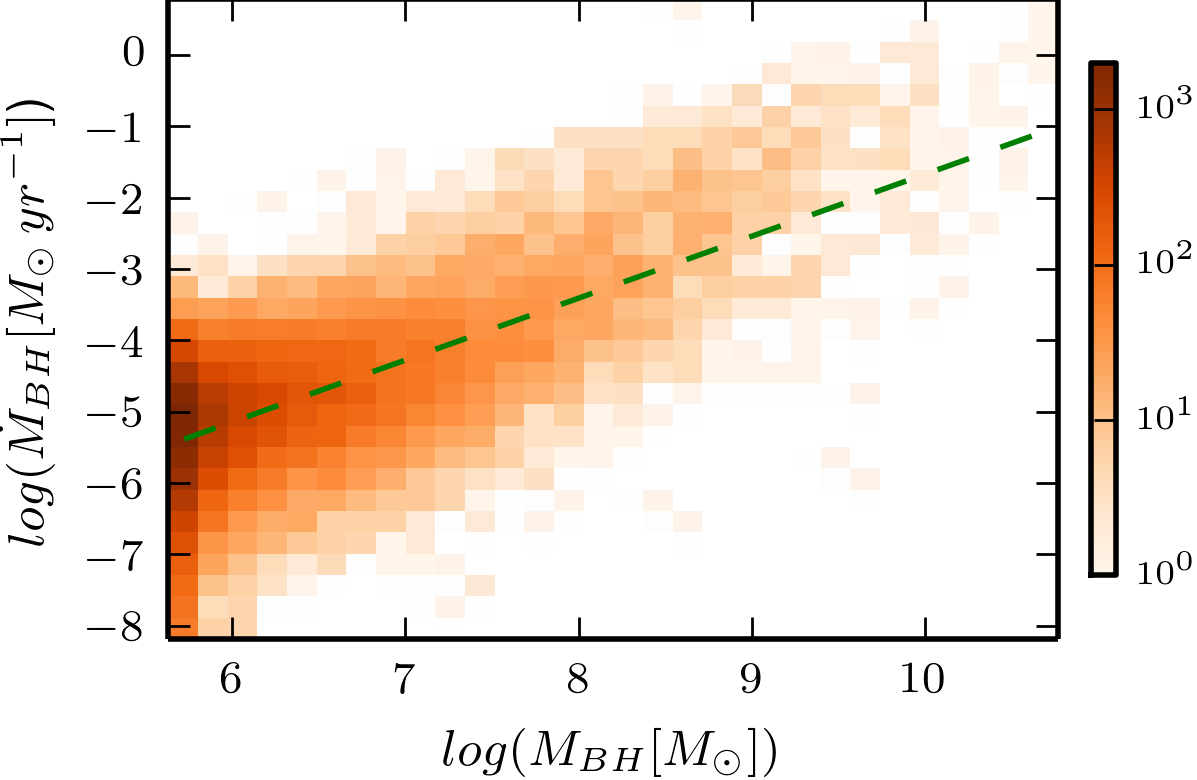
\includegraphics[clip]{Figures/Illustris2_bhpop_hist2d}
\protect\caption{\label{fig:bhpop_hist2d}Black hole accretion rate as a function of
black hole mass for the Illustrist-2 simulation for our sample. The
best-fit power-law relationship between $M$ and $\dot{M}$ is shown
in green. Colors correspond to a two-dimensional density of the same
plot sampled in log space.}
\end{figure}


The fundamental plane of black holes in the local universe from M03
is shown in Figure \ref{fig:Fp} and defined as

\begin{equation}
\log L_{R}=0.6\log L_{x}+0.78\log M_{BH}+7.33
\end{equation}
where the $L_{R}$ is the radio luminosity, $L_{X}$ is the X-ray
luminosity, and $M_{BH}$ is the mass of the black hole. From this
relation, the accretion-powered X-ray luminosity can be expressed
as

\begin{equation}
\log L_{x}=\log M+q\log\dot{m}+K_{2}\;,\label{eq:LxFP}
\end{equation}
where $K_{2}$ is a normalization constant. Depending on the accretion
flow model, the efficiency coefficient $q$ ranges from 0.5 (optically
thick thin disk accretion flow) to 2.3 (advection dominated accretion
flow). The most significant aspect of the fundamental plane is that
it is a correlation which we can apply our general knowledge of galactic
BHs to AGNs and vice versa.
\begin{figure}
\centering{}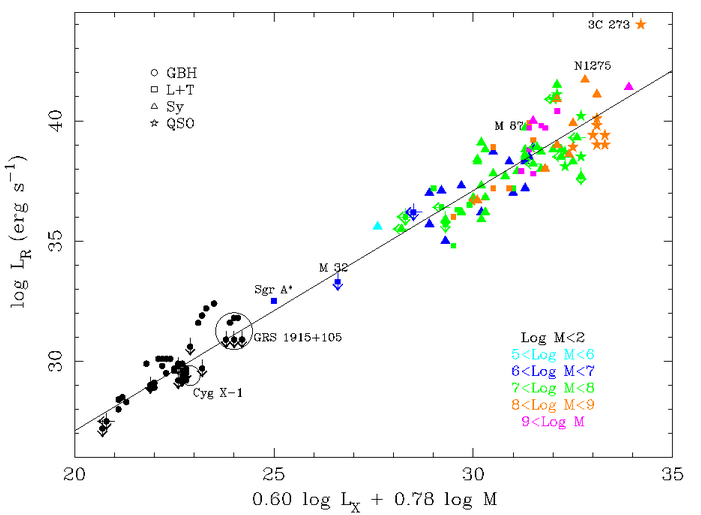
\includegraphics[clip,scale=0.35]{Figures/FP} \protect\caption{\label{fig:Fp}Edge-on view of the fundamental plane from M03 relating
the black hole mass to the radio and X-ray luminosities. Symbols indicate
the type of emission-line galaxy of the host and colors correspond
to the mass of the black hole in units of $\log\left({\rm M}_{\odot}\right)$.
Several well-known galaxies hosting an AGN are listed, as well.}
\end{figure}


The fundamental plane of the BHs relates the mass, X-ray luminosity
and accretion rate. Because the luminosity is not an intrinsic property
of the simulation, it had to be calculated. The calculation of the
luminosity for BH can be approximated by two different models. The
first one takes into account the Eddington luminosity of the BH, which
relates it to the mass, and the second uses the thin disk approximation,
which relates the luminosity to the accretion rate. Both of these
approximations for the luminosity gives the bolometric luminosity.
To get the X-ray luminosity from the bolometric luminosity we use
the \citet{elvis1994atlasof} data sample to calculate a template
. The equation relation from the Elvis template is given by

\begin{equation}
L_{x}=0.1947L_{bol}+1.656\times10^{-15}\;.
\end{equation}


Assuming the BH is only emitting at 10\% off the Eddington luminosity
and by means of the Elvis Template the X-luminosity for the BH is
given by

\begin{equation}
L_{x}=623.04M+1.656\times10^{-15}\;.\label{eq:Lx_propto_m}
\end{equation}
By assuming a thin disk approximation with 10\% efficiency we get
that the X-luminosity for the BH is given by

\begin{equation}
L_{x}=4.64\times10^{19}\dot{M}+1.656\times10^{-15}\;,\label{eq:Lx_propto_mdot}
\end{equation}
for all the cases the masses, accretion rates and luminosities are
measured in $M_{\odot}$, $M_{\odot}s^{-1}$ and $L_{\odot}$. With
equations \ref{eq:Lx_propto_m} and \ref{eq:Lx_propto_mdot} and using
the equation \ref{eq:LxFP}. The fundamental plane equation can be
rewritten in terms of mass, accretion rate, k and q. By means of using
the intrinsic mass to accretion relation, equation \ref{eq:int_relation},
the fundamental plane can be express with only 3 variables.

\begin{multline}
log_{10}(9.03\times10^{18}\dot{M}+1.656\times10^{-15})+1.115log_{10}(\dot{M})\\
-\frac{e}{d}qlog_{10}(\dot{M})+k=0
\end{multline}
\begin{multline}
log_{10}(623.04+\frac{1.656\times10^{-15}}{M})\\
-0.869qlog_{10}(M)+17.855-k=0
\end{multline}


The parameter $q$ holds the information on the properties of the
BH. Hence the adequate value that fits the simulations had to be found.
Using the Newton-Raphson numerical root-finding method for the two
equations and evaluating throw the whole data sample, $q$ is express
in terms of $k$. We find a high correlation between the values of
$q$ and $k$. Since we hope to reproduce the slope $q$ from M03,
which does not provide typical values for $k$, we must approach this
in a rather roundabout manner. We assume that both approximations
for $L_{x}$ are equally good, and will yield similar results, and
combine \ref{eq:Lx_propto_m} and \ref{eq:Lx_propto_mdot} with the
relationship found between $M$ and $\dot{M}$ given by

\begin{multline*}
log_{10}(a_{1}+\frac{b}{M})-dqlog_{10}(M)+eq\\
-log_{10}(a_{2}\dot{M}+b)+\frac{1}{d}log_{10}(\dot{M})-\frac{e}{d}qlog_{10}(\dot{M})=0\;,
\end{multline*}
where $a_{1}$, $a_{2}$, and $b$ are obtained from converting simulation
units to physical units; and $d$ and $e$ are the slope and the intercept
of the power-law found above. We find that $a_{1}=623.04$, $a_{2}=9.03\times10^{18}$,
$b=1.656\times10^{-15}$, $d=0.869$, and $e=-17.855$.\textbf{These
need units.}

A value of $q$ is found for each black hole by inputting values of
$M$ and $\dot{M}$, and solving for $q$ using Newton-Raphson numerical
root-finding. For the distribution of black holes in our Illustris-2
sample, the distribution of $q$ values is shown in \ref{fig:q_nr_hist}.
The distribution of $q$ values obtained is strongly peaked at around
$.068$, with a mean of $.0693$.

\textbf{What does Figure 4 tell us? It's never mentioned.}
\begin{figure}
\centering{}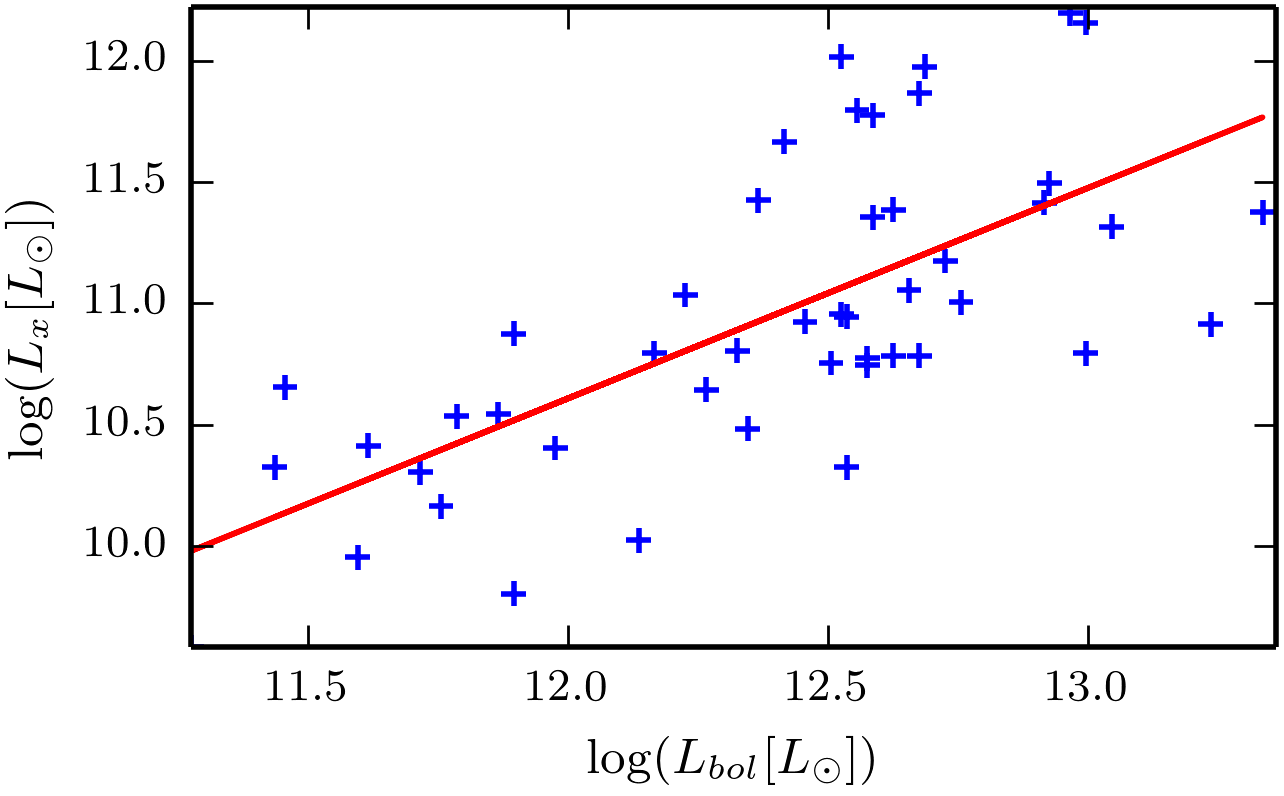
\includegraphics[clip]{Figures/elvis_template} \protect\caption{\label{fig:Elvis_template}The data points from the BH luminosities
over plot with the best-fit linear relation between $L_{x}$ and $L_{bol}$
for the sample.}
\end{figure}
\begin{figure}
\begin{centering}
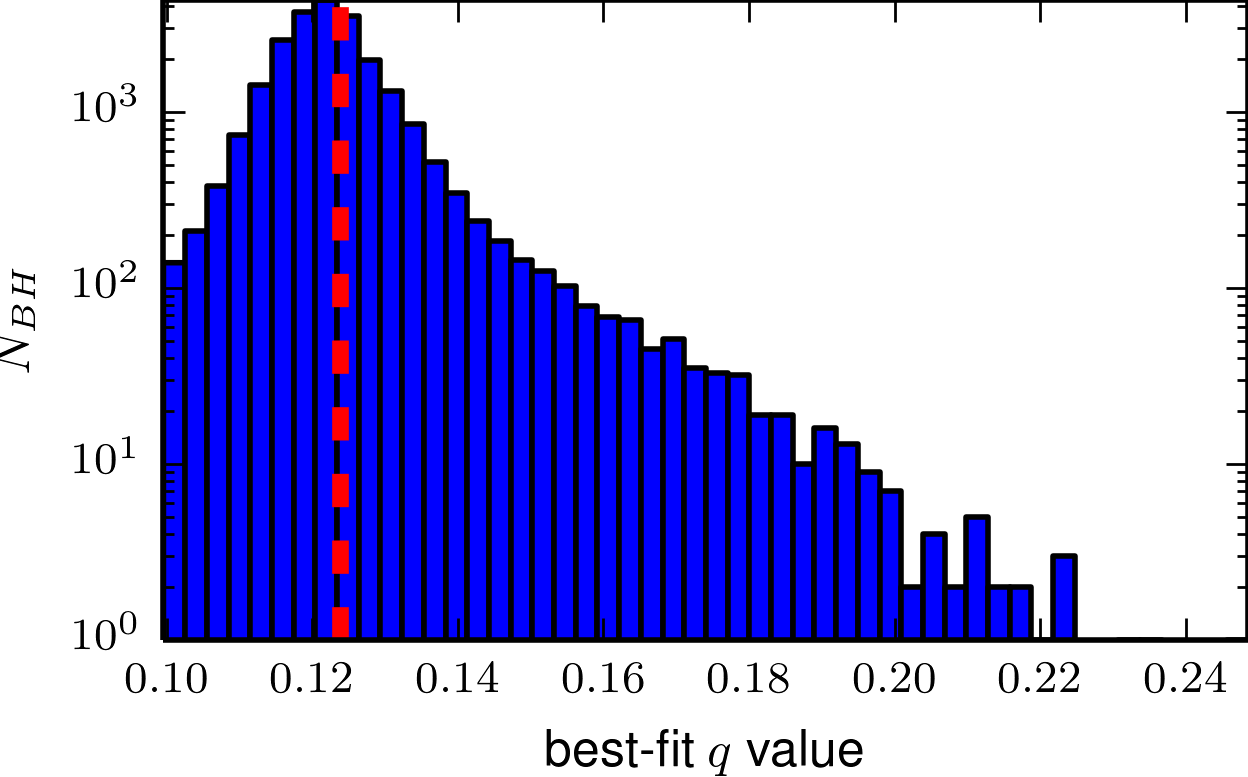
\includegraphics{Figures/q_nr_hist}
\par\end{centering}

\protect\caption{\label{fig:q_nr_hist}A log-histogram of the number of best-fit $q$
values, with one value found per Illustris-2 black hole, using Newton-Raphson
root finding. The maximum likelihood is (SOMEWHERE), with (SOME NUMBER
OF) black holes, and the mean value is $0.693$.}
\end{figure}



\section{Discussion}

\label{sec:discussion}It is well known that the accretion processes
of black holes and the resultant energy deposition into the host galaxy
are necessary ingredients in the evolution of galaxies over cosmic
time. Although we do not understand the causal relationship between
the black hole and its host galaxy, our ability to constrain the mechanisms
responsible are derived principally from simulations of the phenomena.
Using the Illustris-2 simulation, we are able for the first time to
quantify the growth and evolution of supermassive black holes in a
cosmological simulation at the resolution of \textbf{XXX }${\rm M_{\odot}}$.
Using these high-resolution simulation results, we have modelled both
the x-ray and radio luminosities as a function of black hole mass
over the full range present in the Illustris-2 simulation.

In Figure \ref{fig:bhpop_hist2d}, we find that the accretion rate
of black holes with masses less than the median mass of $\mathbf{XXX}{\rm M}_{\odot}$
exhibit accretion rates that differ by \textbf{N} orders of magnitude.
Further, \textbf{XXX\%} exhibit accretion rates less than $10^{-10}\,{\rm M_{\odot}s^{-1}}$
indicating that, on the average, a black hole must accrete for $\mathbf{XX}\,{\rm Gyrs}$
to achieve the median mass. These accretion rates are too low to account
for their masses at $z=0$. For example, a typical low-mass ($10^{7}M_{\odot}$)
black hole accretes at approximately $10^{-12}M_{\odot}s^{-1}$ at
$z=0$. At this rate, such a black hole could only yields a mass of
$\sim10^{5}M_{\odot}$ over the simulation time. Although the high-mass
black holes have generally larger accretion rates in excess of $\dot{M}\approx10^{-10}M_{\odot}s^{-1}$,
the same calculation yields masses of $\sim10^{7}M_{\odot}$ compared
to the actual mass of $\sim10^{9}M_{\odot}$ attained over the simulation
time. This implies that the accretion rates for most of the black
holes in the simulation were likely much larger in the past. This
is consistent with the notion that black hole accretion rates are
tied to the gas fraction in galaxies which was larger at higher redshift.
\textbf{Can we find out when the BH was seeded? I want to make a plot
of seed time vs mass to make this more concrete. Is the linear relation
between mass and $\dot{M}$ known either empirically or from theory?}

\textbf{Talk about Figure 5.}

\begin{figure}
\begin{centering}
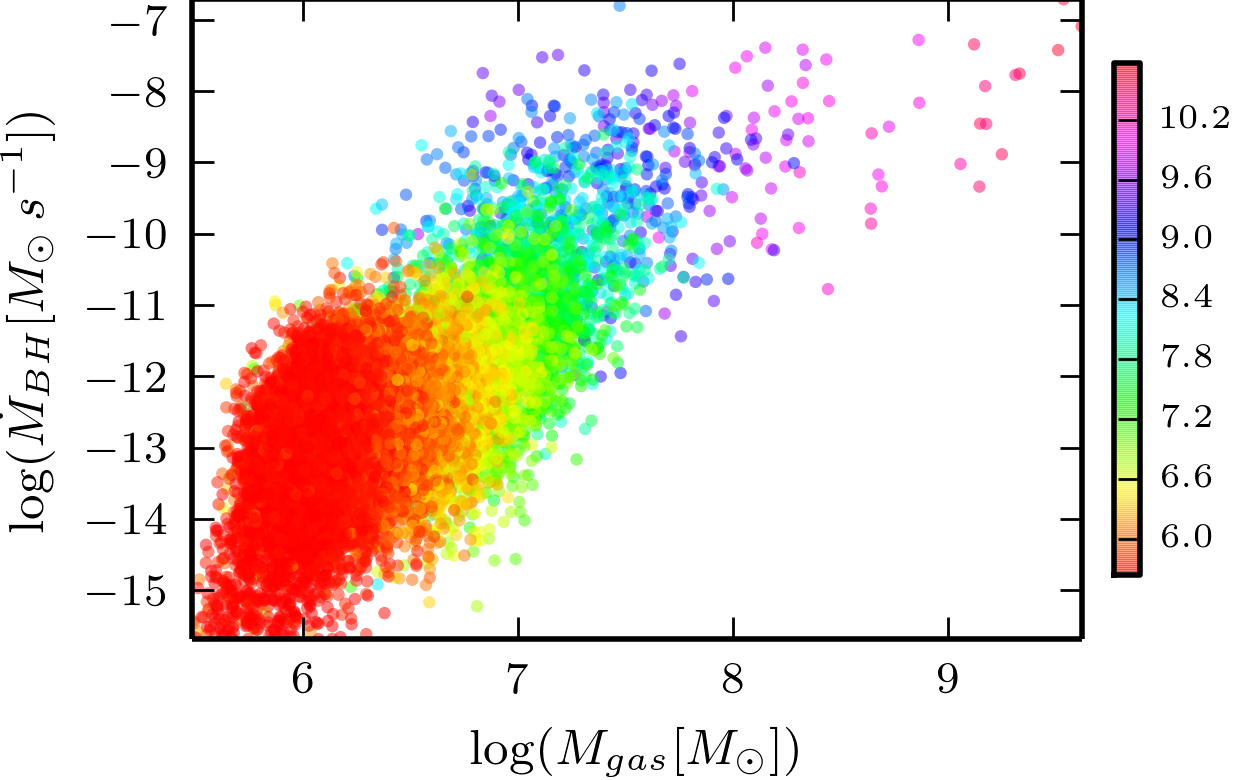
\includegraphics[scale=0.75]{Figures/Mdot_vs_Mgas}
\par\end{centering}

\protect\caption{\label{fig:Mdot_vs_Mgas}Black hole accretion rate of as a function
of the total gas mass in each subhalo for our sample. Colors correspond
to black hole mass. All masses are in units of $\log\left(M_{\odot}\right)$
and the accretion rate is in units $\log\left(M_{\odot}yr^{-1}\right)$.}
\end{figure}



\section{Conclusions}

\label{sec:conclusions}In this work, we have analyzed the complete
of supermassive black holes from the state-of-the-art cosmological
hydrodynamical simulation Illustris-2. Applying well-known models
of black hole phenomena, we calculated the x-ray and radio luminosities
as a function of black hole mass. Using the empirically-derived relation
between these three quantities, we have shown that the 

\bibliographystyle{apj}
\bibliography{BHs_in_Illustris}

\end{document}
